In this section, we discuss the implementation of the different approaches to
solving several subinstances.
As mentioned in the beginning of the chapter, the two
main approaches are to solve a limited amount of subinstances, bounded
by $s(\beta, n)$ for some $\beta$ and a problem size $n$, or to implement a discrete
event simulator that only stores the current state of the network.
First we will discuss the implementation of the tree structure, before we
move on to the two main approaches.

\subsection{Tree Structure}
All trees consists of vertices, and in our specific case, each vertex contains
two sets $\mathcal{M}$ and $\mathcal{Z}$, a solution $x^*$, and a number of
child vertices. To keep vertices as simple as possible, we implement them as
simple \texttt{structs}. Each vertex \texttt{struct} looks like
this:
\begin{verbatim}
struct vertex {
  set<uint16_t> m;
  set<uint16_t> z;
  double* sol;
  vector<struct vertex*> children;
};
\end{verbatim}
A reader familiar with \texttt{C++} might notice that we use
\texttt{set} instead of using a bit vector as we discussed
in Section \ref{ch:tree}, and we will come to that later. Note that
the sets consist of indices of primitive type \texttt{uint16\_t}, which is
short for \texttt{unsigned short int}. That means that the sets are limited to
$2^{16} = 65536$ elements, and therefore also putting a limit to the size
of the QP problems that can be solved. This seems like a reasonable limit
as Goodtech wants to solve problems with $200 - 2000$ variables.
If they need to solve larger problems in the future, it is possible to change
the primitive data type.

As soon as a vertex is defined, we are ready to implement \texttt{mfind}.
Remember that \texttt{mfind} is a modified version of \texttt{find} that tells
us which vertex should be the parent of our potentially new vertex in case it
has a distinct solution.
\texttt{mfind} is defined in two parts. The first part is a driver function
for starting the algorithm on some vertex. The second part is the actual
recursively defined algorithm. These two parts are called \texttt{mfind} and
\texttt{mfindrec}, respectively. We define \texttt{mfind} as follows:
\begin{verbatim}
bool mfind(const set<uint16_t>& m,
struct vertex* v, struct vertex*& ret)
{
  ret = v;
  return mfindrec(m, v, ret);
}
\end{verbatim}
The parameters for \texttt{mfind} are a modifier, a vertex where the search
will begin and an output vertex.
In order to search the whole tree, one would use the root vertex as parameter
\texttt{v}.
The function returns a boolean that changes the meaning of the output vertex.
The function makes a call to \texttt{mfindrec}:
\begin{verbatim}
bool mfindrec(const std::set<uint16_t>& m,
struct vertex* v, struct vertex*& ret)
{
  if (isSubset(m, v->z)) return true;
  for (struct vertex* vi : v->children) {
    if (isSubset(vi->m, m)) {
      ret = vi; 
      bool temp = mfindrec(m, vi, ret);
      if (temp) return true;
    }   
  }   
  return false;
}
\end{verbatim}
It is quite evident from the code that the performance of the \texttt{isSubset}
function is important. In Chapter \ref{ch:tree} we discussed using bit vectors 
to represent sets. We concluded that a simple \texttt{AND} operation would tell
us whether a set was a subset of another set.
We also discussed the possibility of it being more memory efficient than
storing sets in a sparse format where only the indices of each variable was
stored.

Using a bit vector, each set consumes exactly $n$ bits of storage if our
\emph{universe} holds $n$ variables.
Using sets of sparsely stored indices, each set consumes a varying amount of
bits depending on how many variables are in the set. If each index is of data
type \texttt{uint16\_t}, then each index consumes $16$ bits. The trade-off
here is quite clear: If a set contains less than one sixteenth of $n$, then
the sparse format uses less memory. This might actually be the case in a lot
of sets, especially when solving all possible subinstances where the number
of breakdowns are limited by some $\beta$. Consider a very small case where
$n = 200$ and we solve all subinstances
$s(3, 200) = \sum_{j=0}^{3} {\binom{200}{j}} = S$.
With a total number of $S$ sets stored as bit vectors, the memory use for
storing the modifiers is $200S~\textrm{bits} \approx 32~\textrm{megabytes}$.
Whereas, with $S$ sets of sparsely stored indices, the memory use for storing
the modifiers is approximately $8$ megabytes. However, as $\beta$ increases,
the greater the benefits of storing sets in bit vectors become evident. As soon
as $\beta$ becomes greater than 12, bit vectors will use less memory to store all
modifiers. Figure \ref{fig:bmem} shows the ratio of memory used by bit vectors
over memory used by sets of sparsely stored indices where $n = 200$ and
$5 \leq \beta \leq 30$.
\begin{figure}[ht!]
\centering
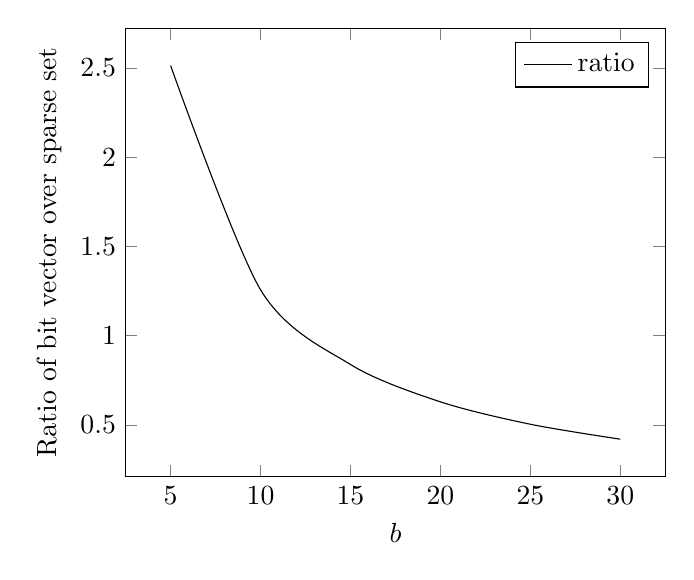
\begin{tikzpicture}
    \begin{axis}[
        legend pos=north east,
        xlabel=$b$,
        ylabel=Ratio of bit vector over sparse set]

        \addplot[black, smooth] plot coordinates {
            (5,  2.51302)
            (10, 1.25686)
            (15, 0.838169)
            (20, 0.628847)
            (25, 0.503276)
            (30, 0.419585)
        };

        \legend{ratio}
    \end{axis}
\end{tikzpicture}

\caption{The ratio of memory use of \texttt{bitset} over \texttt{set} as a
         function of $\beta$.}
\label{fig:bmem}
\end{figure}
Aside from the modifier set, we also have to store the set of variables that
are equal to zero in the optimal solutions of each subinstance. These sets
are more difficult to analyze in terms of memory use, simply because the
cardinality is unknown. However, we do know that $|\mathcal{Z}_k| \geq
|\mathcal{M}_k|$.

With sets of sparsely stored indices, we only need to check the variables
that are actually in the sets in order to determine if a set is a subset
of some set. However, with bit vectors, we need to check $n$ bits---where $n$
is the number of variables in the universe---in order to determine the same.
This means that the \texttt{isSubset} routine will most likely have a different
running time with the two implementations.

One way to find out which of the two are most suited for our need is to perform
a benchmark of the two.
By setting the universe to some size $n$, and generating sets of
random sparsity less than or equal to $n$, we can test how fast
\texttt{isSubset} will run.
We generate random sets as \texttt{bitsets} in \texttt{C++}, storing copies
of these sets in the sparse representation, then testing the performance 
of both implementations of \texttt{isSubset}.
Figure \ref{fig:setspeed}
shows the running time of the two implementations in seconds. Both
implementations were tested on $3000^2$ \texttt{isSubset}-executions, while
increasing $n$.
Codes for the benchmark can be found in Appendix \ref{app:setbench}.
\begin{figure}[ht!]
\centering
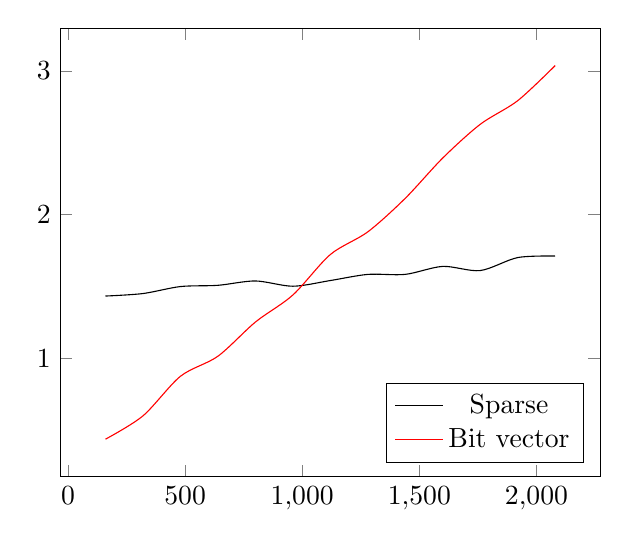
\begin{tikzpicture}
    \begin{axis}[
        legend pos=south east]
%        xlabel=Variables in Universe,
%        ylabel=Seconds]

        \addplot[black, smooth] plot coordinates {
(160, 1.43344)
(320, 1.45082)
(480, 1.49948)
(640, 1.50815)
(800, 1.53846)
(960, 1.50186)
(1120, 1.54138)
(1280, 1.58404)
(1440, 1.58431)
(1600, 1.63973)
(1760, 1.61084)
(1920, 1.70125)
(2080, 1.71173)
        };

        \addplot[red, smooth] plot coordinates {
(160, 0.437256)
(320, 0.599489)
(480, 0.875034)
(640, 1.01462)
(800, 1.25228)
(960, 1.44069)
(1120, 1.72237)
(1280, 1.88017)
(1440, 2.11386)
(1600, 2.39418)
(1760, 2.6287)
(1920, 2.79312)
(2080, 3.03735)
        };

        \legend{Sparse, Bit vector}
    \end{axis}
\end{tikzpicture}

\caption{CPU-seconds used to execute $3000^2$ calls to \texttt{isSubset} on
         randomly generated sets with random sparsity as a function of $n$.}
\label{fig:setspeed}
\end{figure}

We see that the bit vector implementation is much faster than the sparse
implementation on smaller universes. However, the sparse implementation
scales much better than the bit vector implementation when the size of
the universe increases. When it comes to memory, the situation is the same,
except reversed. The sets of sparsely stored indices obviously uses less
memory when $\beta$ is small, i.e. the modifiers are more sparse. However, they
do not scale as nicely as the bit vectors. So the choice relies on what is
most important: memory or speed. Since the nature of this thesis is to
implement a \emph{fast} solver, we give speed a higher priority than memory 
efficiency, so we choose to implement the sets of sparsely stored
indices. That is, in \texttt{C++}, \texttt{set}.

\subsection{Tree Construction}
Because we do not need to store any information about edges in the tree,
we do not need to implement edges as an object of its own. We defined
a vertex \texttt{struct} earlier, having a \texttt{vector} of child
vertices. That means that for each vertex we have, we can reach all children
vertices, children's children vertices and so on, from that vertex.
So, if we have a pointer to the root of a tree, we can reach all vertices
in the tree. Although we earlier defined a tree as an ordered pair
$(V, E)$ of a set of vertices $V$ and a set of edges $E$, we only need a
pointer \texttt{struct vertex*} to our root to access our tree.

The biggest operations in Algorithm \ref{alg:construct} is iterating the power
set of $\left\{1,2,\ldots,n\right\}$. There are lots of combination generators available, so
instead of re-inventing the wheel, we choose a generator that suits our needs.
We need one that is easy to use, and is capable of generating combinations of
a given cardinality. One implementation, similar in use to
\texttt{next\_permutation} in the standard \texttt{C++ STL}, is presented
in~\cite{codeproject}.
Codes from \cite{codeproject} can be found in Appendix
\ref{app:nextcombination}.

The remaining parts of the \texttt{construct}-routine is just running
\texttt{mfind} on each generated modifier, and adding it to the tree
if necessary. Then at the end, return the pointer to the root vertex.
